\section{Graph Databases}
A graph database management system \citep{robinson13} (henceforth, a graph database) is an online database management system with Create, Read, Update, and Delete (CRUD) methods, and is based on graph theory.

Graphs are one of the most efficient and natural way of working with data. Formally speaking a graph is just a collection of vertices and edges. The term \textit{graph theory} been used in centuries, and was first introduced by the Swiss mathematician Leonard Euler (1707-1783) when he in 1736 proved that there does not exist a closed walk that crossed exactly once each of the seven bridges of the river Pregel in Köningsberg, now called Kaliningrad\citep{alexanderson06}. Figure \ref{fig:7bridgesEuler} shows Eulers original drawings from his paper written in 1736 \citep{euler1741} of the bridges in Köningsberg. 

\begin{figure}[H]
  \centering
  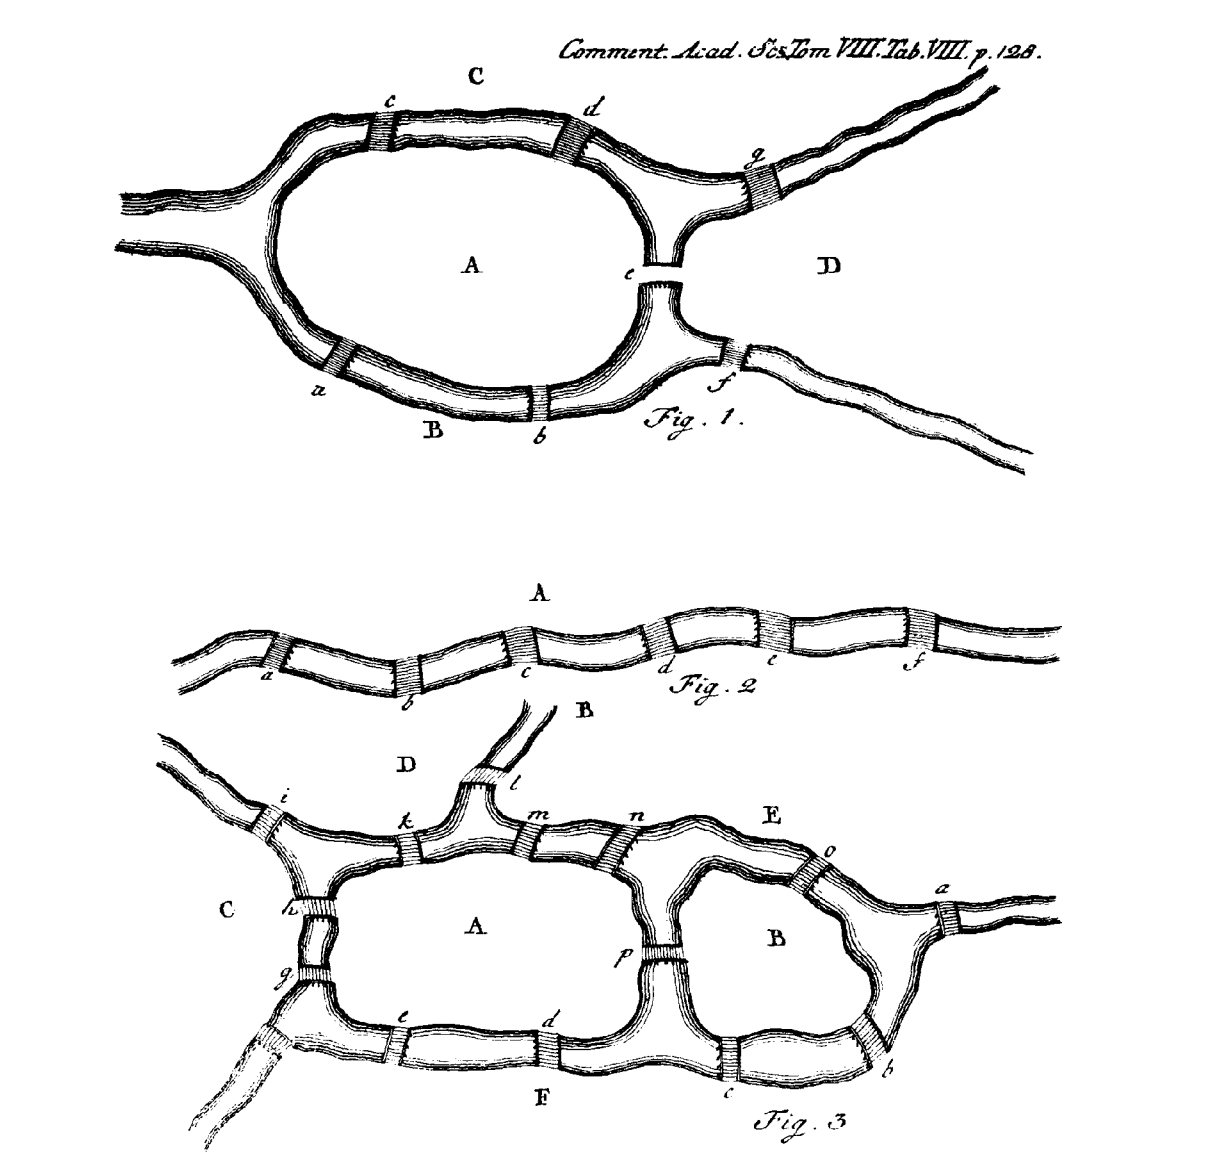
\includegraphics[width=4in]{assets/7bridges-euler.png}
  \caption{Eulers original drawing of the Seven Bridges of Köningsberg} 
  \label{fig:7bridgesEuler}
\end{figure}

Based on the solution of the ``Seven Bridges of Köningsberg''-problem, Euler presented a theorem that states that if the graph is planar and connected, and if \textit{v} is the number of vertices, \textit{e} is the number of edges and \textit{f} is the number of faces (regions between edges of a plane graph that does not have any edges in it), then 
\newline
\newline
\centerline{$v-e+f=2$}
\newline
\newline
This means, with respect to the ``Seven Bridges of Köningsberg''-problem, that if it does not exists a path in the graph that lets you visit every node using every edge exactly once, the sum will not be 2. We have illustrated the bridges in Köningsberg as a graph in figure \ref{fig:7bridgesIllustration} and simplified the illustration in figure \ref{fig:7bridgesSimplification}. We see that the graph consists of 4 vertices, 7 edges and 4 faces. The faces are specified with numbers 1-4 in figure \ref{fig:7bridgesSimplification}. If we use the theorem described above we see that $4-7+4\neq2$, which is consistent with Eulers proof from 1736. 

\begin{figure}[H]
  \centering
  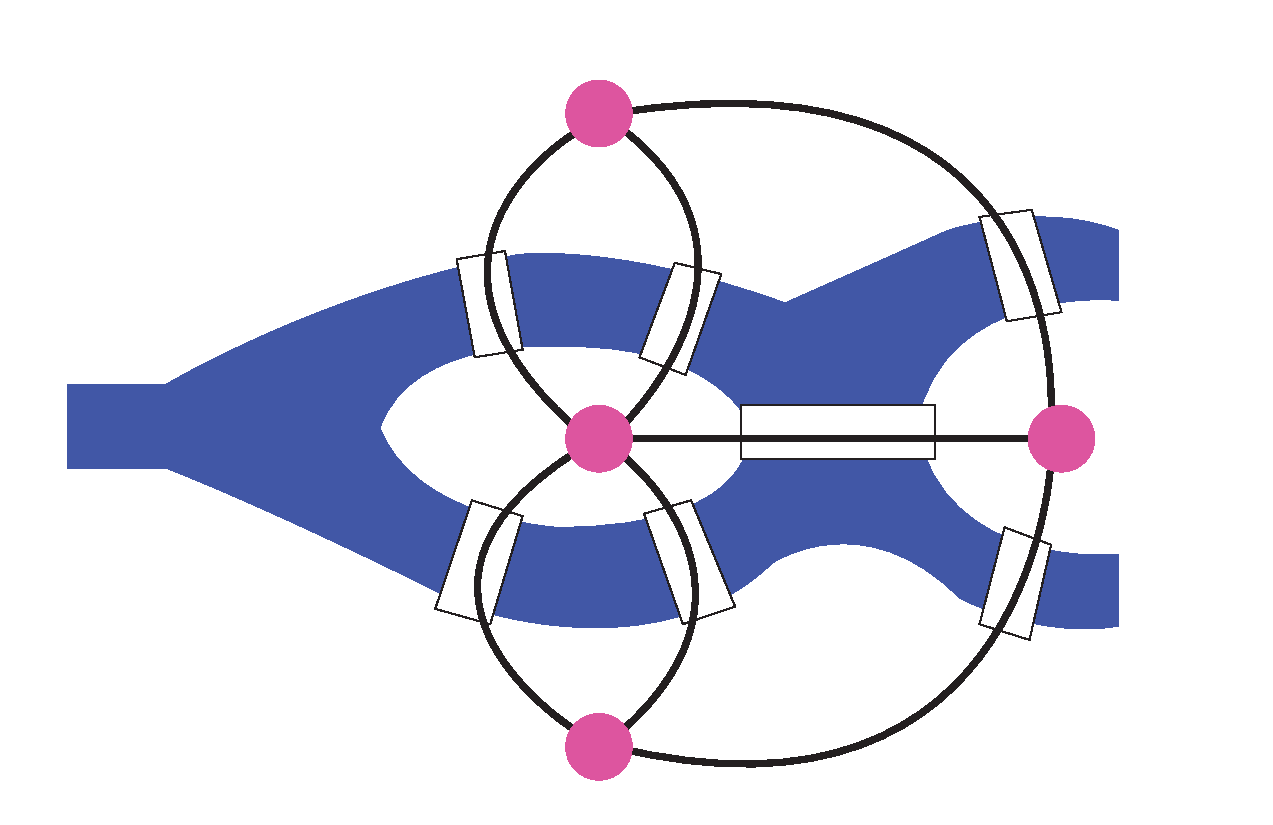
\includegraphics[width=4in]{assets/7bridges.pdf}
  \caption{Illustration of the Seven Bridges of Köningsberg as a graph} 
  \label{fig:7bridgesIllustration}
\end{figure}

\begin{figure}[H]
  \centering
  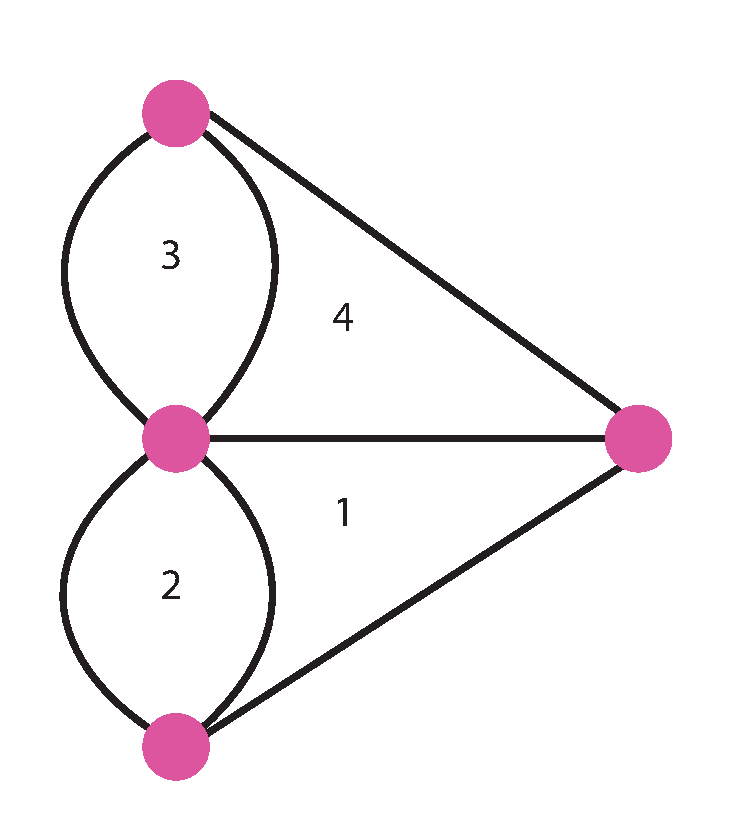
\includegraphics[width=2in]{assets/7bridges2.pdf}
  \caption{The simplified graph of the Seven Bridges of Köningsberg} 
  \label{fig:7bridgesSimplification}
\end{figure}

Graph databases consists of nodes, edges, and properties to represent and store data:
\begin{itemize}
\item Nodes represent entities, such as people, accounts or bus stops
\item properties are relevant information that relate to the nodes, and 
\item edges are the lines that connect the nodes and properties, defining the relationship between them. Most of the information is stored in the edges, for instance the travel time or travel demand between to bus stops. 
\end{itemize}

Graph databases are a powerful tool for graph-like queries. Applications of graph databases range from calculating routes between locations in an abstract network such as a road or rail network, airspace network, or logistical network to spatial operations such as find all points of interest in a bounded area, find the center of a region, and calculate the intersection between two or more regions \citep{robinson13}.

%Graph theory is a mature and well-understood field of study concerning the nature of
%networks (or from our point of view, connected data)\citep{robinson13}. 



%A graph database management system (henceforth, a graph database) is an online database management system with Create, Read, Update, and Delete (CRUD) methods that expose a graph data model. 

%It uses graph structures for semantic queries. It is a storage system where every element contains a direct pointer to its neighbor elements and no index lookups are necessary. 

\par %Skrives om litt

%Relational and NOSQL databases lack relationships \citep{robinson13}. Compared to relational databases, are graph databases often faster for associative data sets[Wikipedia:P], and map more directly to the structure of object-oriented applications. They can scale more naturally to large data sets as they do not typically require extensive join operations. As they depend less on a inflexible schema, they are more suitable to manage changing data with evolving schema's.

\par
%Graph databases are a powerful tool for graph-like queries, for instance computing the shortest path between to nodes in the graph!!! Other graph-like queries can be performed over a graph database in a natural way (for example graph's diameter computations or community detection).

%Geospatial is the original graph use case: Euler solved the Seven Bridges of Königsberg problem by positing a mathematical theorem that later came to form the basis of graph theory. Geospatial applications of graph databases range from calculating routes between locations in an abstract network such as a road or rail network, airspace network, or logistical network to spatial operations such as find all points of interest in a bounded area, find the center of a region, and calculate the intersection between two or more regions. \citep{neo13}
%Geospatial operations depend upon specific data structures, ranging from simple weighted and directed relationships, through to spatial indexes, such as R-Trees, which represent multidimensional properties using tree data structures. As indexes, these data structures naturally take the form of a graph, typically hierarchical in form, and as such they are a good fit for a graph database. Because of the schema-free nature of graph databases, geospatial data can reside in the database beside other kinds of data—social network data, for example—allowing for complex multidimensional querying across several domains. Geospatial applications of graph databases are particularly relevant in the areas of telecommunications, logistics, travel, timetabling, and route planning \citep{neo13}

\par

%\textit{Denne er foreløpig kopiert fra Wikipedia: }%Skrives om 
%Compared with relational databases, graph databases are often faster for associative data sets[citation needed], and map more directly to the structure of object-oriented applications. They can scale more naturally to large data sets as they do not typically require expensive join operations. As they depend less on a rigid schema, they are more suitable to manage ad hoc and changing data with evolving schema's. Conversely, relational databases are typically faster at performing the same operation on large numbers of data elements.


\subsection{Neo4j}
Neo4J \citep{website:neo4j} is a native graph database, native graph storage that is optimized and designed for
storing and managing graphs.

and is a success way to store a transport graph. It is known for extremely fast traversals of relationships. Neo4J can be easily constructed to a transit network. It is fast finding shortest path (by Dijkstra's algorithm), and it is easy to change the database via the REST API. 

Neo4J is a highly scalable open source graph database that supports ACID, has high-availability clustering for enterprise deployments, and comes with a web-based administration tool that includes full transaction support and visual node-link graph explorer. Neo4j is accessible from most programming languages using its built-in REST web API interface. Neo4j is the most popular graph database in use today.[10]

Advantages:
\begin{itemize} 
\item Flexibility: model, develop and visualize the world as you experience it. Its simply nodes and relationships. 
\item Performance: Hyper-connectivity at speed. 
\item Scalability: Scales up and out, supporting tens of billions of nodes and relationships, and hundred of thousands of ACID transactions per seconds. 
\item Speed: Able to search trough millions of connections per second, with real time queries that stay fast even as your database grows. 
\end{itemize}

\subsubsection{Dijkstra's algorithm}
Dijkstra  is used  by Neo4j to find the shortest path between two nodes in the graph. Dijkstra’s algorithm is mature, having been published in 1956, and thereafter widely studied and optimized by computer scientists.\citep{neo13}. Dijkstra’s algorithm is quite efficient because it computes only the lengths of a relatively small subset of the possible paths through the graph. Dijkstra is often used to find real-world shortest paths (e.g., for navigation). It behaves as follows:
\begin{enumerate}
\item Pick the start and end nodes, and add the start node to the set of solved nodes (that is, the set of nodes with known shortest path from the start node) with value 0 (the start node is by definition 0 path length away from itself).
\item From the starting node, traverse breadth-first to the nearest neighbors and record the path length against each neighbor node.
\item Take the shortest path to one of these neighbors (picking arbitrarily in the case of ties) and mark that node as solved, because we now know the shortest path from the start node to this neighbor.
\item From the set of solved nodes, visit the nearest neighbors (notice the breath-first progression) and record the path lengths from the start node against these new neighbors. Don’t visit any neighboring nodes that have already been solved, because we know the shortest paths to them already.
\item Repeat steps 3 and 4 until the destination node has been marked solved.
\end{enumerate}


%\begin{itemize}
%\item Native graph database. 
%\item Property graph. 
%\item Made for real time queries. 
%\item Really fast traversals of relations.
%\item Neo4J has an API that supports traversing - finding shortest path - can weight edges, nodes -
%\end{itemize}
%//en korteste vei mellom n og m men max lengde 3
%match p = shortestPath ( (n) - [*...3]--(m)) return p
%(Vekte kanter: Neo44J har et API som støtter traversering, Dijkstras er innebyd ++ som lar deg vekte kanter - hva er raskeste vei ++)

%Neo4J can be used to evaluate routes after the ants have created route sets.